\documentclass[aspectratio=169]{beamer}
\usetheme{default}
\setbeamertemplate{navigation symbols}{}
\usecolortheme{structure}\setbeamercolor{structure}{fg=black}
\usepackage{amsmath}
\usefonttheme[onlymath]{serif}
\usepackage{tikz}
\usetikzlibrary{arrows.meta}

\begin{document}

\begin{frame}{What should the power meter show?}

\begin{columns}[c]

% ---- Left: simple circuit ------------------------------------------------
\begin{column}{0.37\textwidth}
\centering
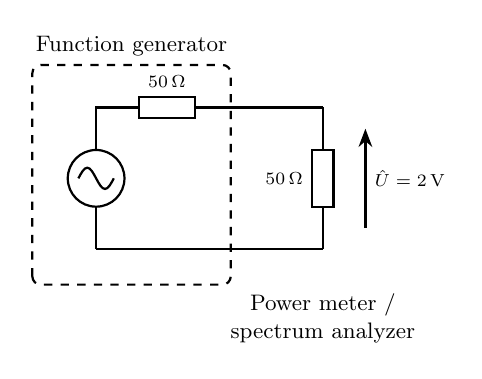
\begin{tikzpicture}[thick, font=\small, scale=0.9, transform shape]
  % generator (dashed outline)
  \draw[dashed, rounded corners=3pt] (-0.9,-1.5) rectangle (1.9,1.6);
  \node[above] at (0.5,1.6) {Function generator};

  % sine source
  \draw (0,-1) -- (0,-0.4);
  \draw (0,0) circle (0.4);
  \draw (-0.25,0) sin (-0.125,0.15) cos (0,0) sin (0.125,-0.15) cos (0.25,0);
  \draw (0,0.4) -- (0,1) -- (0.6,1);

  % internal 50 ohm
  \draw (0.6,0.85) rectangle (1.4,1.15);
  \node[above, font=\scriptsize] at (1.0,1.15) {$50\,\Omega$};
  \draw (1.4,1) -- (3.2,1);
  \draw (0,-1) -- (3.2,-1);

  % meter = 50 ohm load
  \draw (3.05,0.4) rectangle (3.35,-0.4);
  \draw (3.2,1) -- (3.2,0.4);
  \draw (3.2,-0.4) -- (3.2,-1);
  \node[left, font=\scriptsize] at (3.05,0) {$50\,\Omega$};
  \node[below, align=center] at (3.2,-1.5) {Power meter /\\spectrum analyzer};

  % voltage across the load
  \draw[-{Stealth}] (3.8,-0.7) -- (3.8,0.7);
  \node[right, font=\scriptsize] at (3.8,0) {$\hat U = 2\,\mathrm{V}$};
\end{tikzpicture}
\end{column}

% ---- Right: the math -----------------------------------------------------
\begin{column}{0.61\textwidth}
\begin{align*}
  \hat U &= 2\,\mathrm{V}
    \quad \text{\scriptsize (amplitude, $4\,\mathrm{V_{pp}}$)}\\[4pt]
  U_{\mathrm{rms}} &= \frac{\hat U}{\sqrt 2} \approx 1{.}41\,\mathrm{V}
    \quad \text{\scriptsize (sine)}\\[4pt]
  P &= \frac{U_{\mathrm{rms}}^2}{R} = \frac{1{.}41^2}{50} = 40\,\mathrm{mW}\\[4pt]
  P_{\mathrm{dBm}} &= 10\log_{10}\!\left(\frac{40\,\mathrm{mW}}{1\,\mathrm{mW}}\right)
    \approx \boxed{16\,\mathrm{dBm}}
\end{align*}

\vspace{2pt}
{\scriptsize
Generator set to \textbf{50\,\boldmath$\Omega$ load}: the 2\,V is what
actually reaches the meter.\\[2pt]
Set to \textbf{High-Z} instead? Only half the voltage reaches the meter
$\Rightarrow$ $-6\,\mathrm{dB}$ $\Rightarrow$ \textbf{10\,dBm}.
}
\end{column}

\end{columns}

\end{frame}

\end{document}
